\documentclass[answers]{exam} % Clase para exámenes con respuestas
\usepackage[english,spanish]{babel} % Soporte para inglés y español
\usepackage[autostyle]{csquotes} % Manejo de citas
\usepackage{amsmath, amssymb} % Paquetes para matemáticas avanzadas
\usepackage{graphicx} % Inclusión de gráficos
\usepackage{wrapfig}
\usepackage{enumitem} % Personalización de listas enumeradas
\usepackage[letterpaper,top=2cm,bottom=2cm,left=3cm,right=3cm,marginparwidth=1.75cm]{geometry} % Configuración de márgenes
\usepackage[colorlinks=true, allcolors=blue]{hyperref} % Enlaces con color
\usepackage{tikz}
\usepackage{pgfplots}
\usepackage{array}   % for adjusting row height
\renewcommand{\arraystretch}{1.5} % adjust the vertical spacing between rows

\renewcommand{\solutiontitle}{\noinde\par\noindent} % Personalización del título de respuestas
\renewcommand{\familydefault}{\sfdefault}

% Configuración de encabezado y pie de página
\pagestyle{headandfoot}
\firstpageheader{Universidad de Bolívar}{}{Noviembre 19, 2024} 
\runningheader{Universidad de Bolívar}{}{Física}
\firstpagefooter{}{\thepage}{}
\runningfooter{}{\thepage}{}

\begin{document}

\begin{center}
	\large\textbf{Trabajo Autónomo 2.11 - Fundamentos de Física para Ingeniería}\\[1em]
	\large Segundo Ciclo \enquote*{A} - Ingeniería de Software\\[1em]
\end{center}

\vspace{0.5cm}
\noindent
\large\textbf{Tema:} DIELÉCTRICOS Y CONDENSADORES \\
\large\textbf{Estudiante:} Ariel Alejandro Calderón
\vspace{0.5cm}

\begin{questions}

	\question \textbf{Se tiene un sistema formado por tres capacitores, como se muestra en la figura. Entre los terminales A y B de dicho sistema se ha aplicado una diferencia de potencial de 200 V. Determine:}
	\begin{enumerate}[label=\alph*. ]
		\item  La capacitancia equivalente del sistema.
		\item  La carga y la diferencia de potencial en cada capacitor.
	\end{enumerate}

	\begin{minipage}{\textwidth}
		\centering
		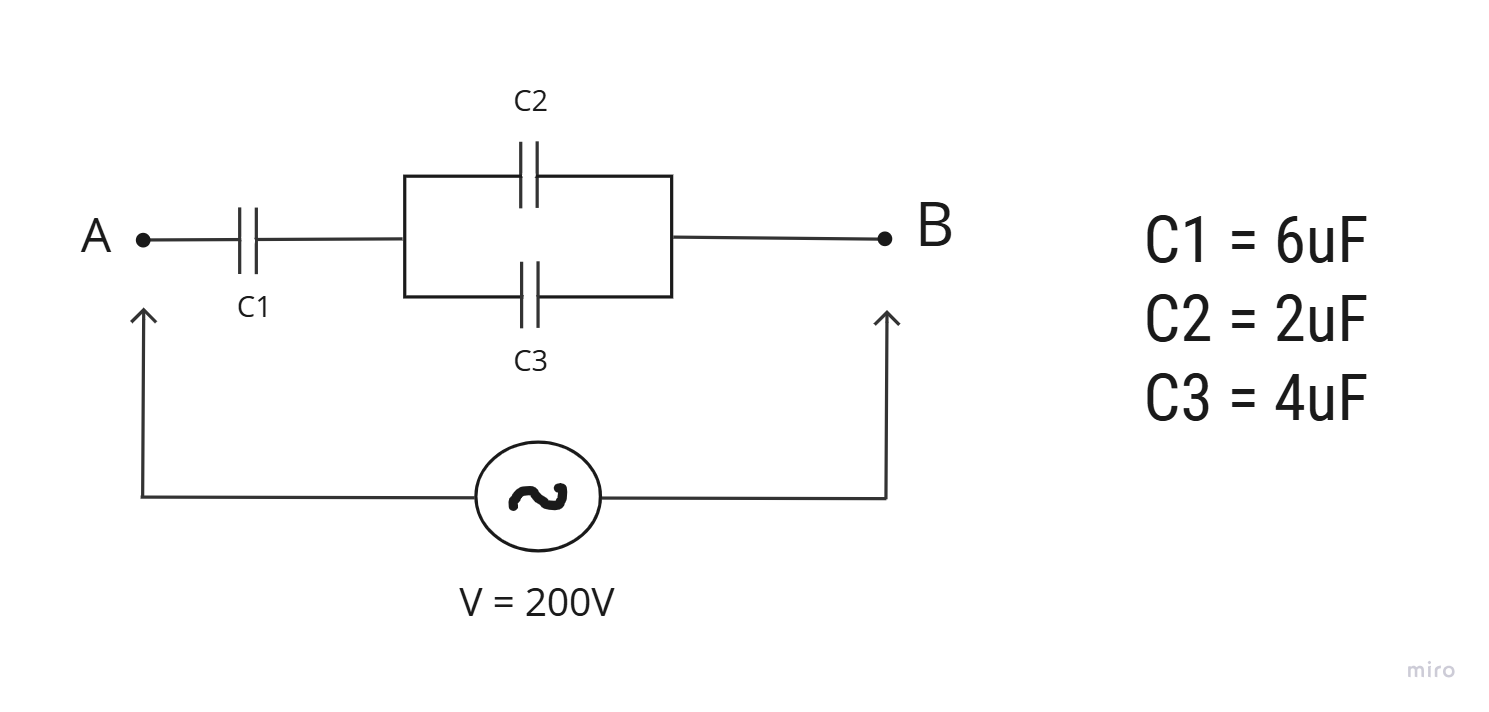
\includegraphics[width=0.9\textwidth]{public/g1.png}\\
	\end{minipage}
	\begin{parts}

		\part{Capacitancia equivalente}\\

		\textbf{Capacitores en paralelo:}
		\[
			C_{23} = C_2 + C_3 = 2 \mu F + 4 \mu F = 6 \mu F
		\]

		\textbf{Capacitores en serie:}
		\[
			\frac{1}{C_{eq}} = \frac{1}{C_1} + \frac{1}{C_{23}} = \frac{1}{6 \mu F} + \frac{1}{6 \mu F} = \frac{1}{3 \mu F}
		\]

		Por lo tanto, $C_{eq} = 3 \mu F$

		\part{Carga y la diferencia de potencial en cada capacitor}\\

		Carga total:
		\[
			Q = C_{eq} \cdot V = 3 \mu F \cdot 200 V = 600 \mu C
		\]

		Diferencia de potencial en C1:
		\[
			V_1 = \frac{Q}{C_1} = \frac{600 \mu C}{6 \mu F} = 100 V
		\]

		Diferencia de potencial en C2 y C3:
		\[
			V_2 = V_3 = V - V_1 = 200 V - 100 V = 100 V
		\]

		Carga en C2 y C3:
		\[
			Q_2 = C_2 \cdot V_2 = 2 \mu F \cdot 100 V = 200 \mu C
		\]
		\[
			Q_3 = C_3 \cdot V_3 = 4 \mu F \cdot 100 V = 400 \mu C
		\]


	\end{parts}

	\vspace{0.5cm}

	\question \textbf{Se tienen dos capacitores planos conectados entre sí, y se sabe que el potencial de cada uno es 200 V. Si se introduce un dieléctrico de permitividad relativa \(\varepsilon_r = 3\) entre las placas del capacitor \(C_1\), calcule la carga y el potencial de cada capacitor si sus capacitancias antes de introducir el dieléctrico eran \(C_1 = 0.05 \, \mu F\) y \(C_2 = 0.1 \, \mu F\).}

	\begin{parts}
		\part \textbf{Carga en cada capacitor:} \\
		La carga en cada capacitor se puede calcular utilizando la fórmula:
		\[
			\boxed{Q = C \cdot V}
		\]
		Donde \(C\) es la capacitancia de cada capacitor y \(V\) es el potencial aplicado.

		- Para el capacitor \(C_1\) con dieléctrico, la capacitancia aumenta debido a la introducción del dieléctrico de permitividad relativa \(\varepsilon_r = 3\). La nueva capacitancia será:
		\[
			C_1' = C_1 \cdot \varepsilon_r = 0.05 \, \mu F \times 3 = 0.15 \, \mu F
		\]
		- Para el capacitor \(C_2\), no se introduce dieléctrico, por lo que su capacitancia permanece igual: \(C_2 = 0.1 \, \mu F\).

		La carga \(Q_1\) en el capacitor \(C_1\) se calcula como:
		\[
			Q_1 = C_1' \cdot V = 0.15 \, \mu F \cdot 200 \, \text{V} = 30 \, \mu C
		\]
		Y la carga \(Q_2\) en el capacitor \(C_2\) se calcula como:
		\[
			Q_2 = C_2 \cdot V = 0.1 \, \mu F \cdot 200 \, \text{V} = 20 \, \mu C
		\]

		\part \textbf{Potencial en cada capacitor:} \\
		El potencial en cada capacitor puede calcularse a partir de la carga y la capacitancia utilizando la fórmula:
		\[
			\boxed{V = \frac{Q}{C}}
		\]
		Dado que los capacitores están conectados entre sí, el potencial total se distribuye entre ellos dependiendo de sus capacitancias.
		- Para \(C_1\) con dieléctrico, el potencial será:
		\[
			V_1 = \frac{Q_1}{C_1'} = \frac{30 \, \mu C}{0.15 \, \mu F} = 200 \, \text{V}
		\]
		- Para \(C_2\), el potencial será:
		\[
			V_2 = \frac{Q_2}{C_2} = \frac{20 \, \mu C}{0.1 \, \mu F} = 200 \, \text{V}
		\]
	\end{parts}

	\begin{figure}[h]
		\centering
		\begin{tikzpicture}

			% Dibujo del capacitor C1 con dieléctrico
			\draw[thick] (0,0) rectangle (2,3);
			\draw[thick] (0,3) -- (2,3);
			\draw[thick] (0,0) -- (2,0);
			\draw[fill=gray!20] (0.2,0.2) rectangle (1.8,2.8); % dieléctrico dentro de C1
			\node at (1,2.5) {C\textsubscript{1}};

			% Dibujo del capacitor C2
			\draw[thick] (4,0) rectangle (6,3);
			\draw[thick] (4,3) -- (6,3);
			\draw[thick] (4,0) -- (6,0);
			\node at (5,2.5) {C\textsubscript{2}};

			% Placas de conexión
			\draw[thick] (2,1.5) -- (4,1.5);

			% Etiquetas
			\node at (1,-0.5) {Dieléctrico (\(\varepsilon_r = 3\))};
			\node at (5,-0.5) {Sin dieléctrico};

		\end{tikzpicture}
	\end{figure}

	\question \textbf{Dentro de un capacitor plano cuyas placas tienen un área de \(300 \, \text{cm}^2\) y están separadas por una distancia \(d = 1 \, \text{cm}\), se introduce un dieléctrico que ocupa todo su volumen interior, de manera que su capacitancia ahora toma el valor de \(C = 0.053 \, \text{pF}\). Determine la permitividad relativa del dieléctrico.}

	La capacitancia de un capacitor con dieléctrico está relacionada con la capacitancia sin dieléctrico por la siguiente fórmula:
	\[
		\boxed{C = C_0 \cdot \varepsilon_r}
	\]
	donde:\\
	- \(C_0\) es la capacitancia sin dieléctrico.\\
	- \(\varepsilon_r\) es la permitividad relativa del dieléctrico.\\

	La capacitancia sin dieléctrico, \(C_0\), se puede calcular utilizando la fórmula para la capacitancia de un capacitor plano:
	\[
		\boxed{C_0 = \frac{\varepsilon_0 A}{d}}
	\]
	donde:\\
	- \(\varepsilon_0 = 8.854 \times 10^{-12} \, \text{F/m}\) es la permitividad del vacío.\\
	- \(A = 300 \, \text{cm}^2 = 3 \times 10^{-2} \, \text{m}^2\) es el área de las placas.\\
	- \(d = 1 \, \text{cm} = 10^{-2} \, \text{m}\) es la distancia entre las placas.\\

	Sustituyendo:
	\[
		C_0 = \frac{(8.854 \times 10^{-12}) (3 \times 10^{-2})}{10^{-2}} = 2.6562 \times 10^{-12} \, \text{F} = 2.6562 \, \text{pF}
	\]

	\[
		\varepsilon_r = \frac{C}{C_0} = \frac{0.053 \, \text{pF}}{2.6562 \, \text{pF}} \approx 20
	\]

	Por lo tanto, la permitividad relativa del dieléctrico es \(\varepsilon_r \approx 20\).

	\begin{figure}[h]
		\centering
		\begin{tikzpicture}

			% Dibujo del capacitor con dieléctrico
			\draw[thick] (0,0) rectangle (4,3); % Contorno del capacitor
			\draw[thick] (0,3) -- (4,3);
			\draw[thick] (0,0) -- (4,0);
			\draw[fill=gray!20] (0.2,0.2) rectangle (3.8,2.8); % Dieléctrico dentro del capacitor
			\node at (2,2.5) {Capacitor};

			% Líneas de voltaje
			\draw[thick, thick] (-1, 1.5) -- (-0.2, 1.5);
			\draw[thick, thick] (4.2, 1.5) -- (5, 1.5);

			% Etiquetas del área y separación
			\node at (2, -0.5) {Área = \(300 \, \text{cm}^2\)};
			\node at (2, 3.5) {Separación \(d = 1 \, \text{cm}\)};
			\node at (2.2, 2) {Dieléctrico};

		\end{tikzpicture}

	\end{figure}
	\newpage
	\question \textbf{La intensidad de corriente en el circuito varía de acuerdo con la ecuación \(I = I_0 e^{-kt}\). Halle la cantidad de carga que atraviesa una sección del conductor en los dos primeros segundos. Tome \(k = 0.5 \, \text{s}^{-1}\) y \(I_0 = 0.2 \, \text{A}\).}



	La cantidad de carga \(Q\) que atraviesa una sección del conductor en un intervalo de tiempo \([0, t]\) se puede obtener integrando la corriente \(I(t)\) con respecto al tiempo:

	\[
		\boxed{Q = \int_0^t I(t) \, dt = \int_0^t I_0 e^{-kt} \, dt}
	\]

	Sustituyendo los valores dados, tenemos que \(I_0 = 0.2 \, \text{A}\), \(k = 0.5 \, \text{s}^{-1}\), y \(t = 2 \, \text{s}\):

	\[
		Q = \int_0^2 0.2 e^{-0.5 t} \, dt
	\]

	La integral de \(e^{-kt}\) es \(-\frac{1}{k} e^{-kt}\), por lo tanto:

	\[
		Q = 0.2 \left[ -\frac{1}{0.5} e^{-0.5 t} \right]_0^2  =  0.2 \left( -2 e^{-1} + 2 e^0 \right) = 0.2 \left( -\frac{2}{e} + 2 \right)
	\]

	Usando \(e \approx 2.718\), tenemos:

	\[
		Q = 0.2 \left( -\frac{2}{2.718} + 2 \right) \approx 0.2 \left( -0.735 + 2 \right) \approx 0.2 \cdot 1.265 = 0.253 \, \text{C}
	\]

	Por lo tanto, la cantidad de carga que atraviesa la sección del conductor en los primeros 2 segundos es aproximadamente:

	\[
		Q \approx 0.253 \, \text{C}
	\]

	\begin{figure}[h]
		\centering
		\begin{tikzpicture}
			\begin{axis}[
					width=10cm, height=6cm, % Tamaño del gráfico
					xlabel={Tiempo (\(t\) [s])}, % Etiqueta del eje x
					ylabel={Intensidad de corriente (\(I\) [A])}, % Etiqueta del eje y
					domain=0:3, % Dominio del tiempo
					samples=100, % Número de muestras para mayor suavidad
					grid=both, % Añadimos una cuadrícula
					legend pos=outer north east, % Posición de la leyenda
					xtick={0,1,2,3}, % Posiciones de los ticks en el eje x
					ytick={0,0.05,0.1,0.15,0.2} % Posiciones de los ticks en el eje y
				]
				% Gráfico de la corriente I = I0 * e^(-kt)
				\addplot[blue, thick] {0.2 * exp(-0.5*x)};
				\addlegendentry{\(I(t) = 0.2 \cdot e^{-0.5t}\)} % Leyenda

			\end{axis}
		\end{tikzpicture}

	\end{figure}


	\question \textbf{Un conductor cilíndrico de sección transversal \(A = 0.01 \, \text{cm}^2\) está formado por dos conductores, de hierro y cobre, como se muestra en la figura. Las resistividades de los metales son \(\delta_{\text{Cu}} = 1.75 \times 10^{-8} \, \Omega \, \text{m}\) y \(\delta_{\text{Fe}} = 9.8 \times 10^{-8} \, \Omega \, \text{m}\). La longitud del conductor compuesto es 2.5 m. Entre los extremos se aplica una diferencia de potencial de 1.5 V. Halle:}
	\begin{enumerate}[label=\alph*. ]
		\item  La resistencia total del conductor.
		\item  La intensidad de corriente por cada conductor.
		\item  El valor de la intensidad del campo eléctrico en cada conductor.
	\end{enumerate}

	\begin{parts}
		\part \textbf{La resistencia total del conductor.}

		La resistencia de un conductor se calcula mediante la fórmula:

		\[
			\boxed{R = \delta \frac{L}{A}}
		\]

		Donde:\\
		- \(\delta\) es la resistividad del material,\\
		- \(L\) es la longitud del conductor,\\
		- \(A\) es el área de la sección transversal.\\

		La resistencia total \(R_{\text{total}}\) es la resistencia equivalente de dos resistores en paralelo. Si las resistencias de los conductores de cobre y hierro son \(R_{\text{Cu}}\) y \(R_{\text{Fe}}\) respectivamente, la resistencia total será:

		\[
			\boxed{\frac{1}{R_{\text{total}}} = \frac{1}{R_{\text{Cu}}} + \frac{1}{R_{\text{Fe}}}}
		\]

		La resistencia del cobre es:

		\[
			R_{\text{Cu}} = \delta_{\text{Cu}} \frac{L}{A_{\text{Cu}}}
		\]

		La resistencia del hierro es:

		\[
			R_{\text{Fe}} = \delta_{\text{Fe}} \frac{L}{A_{\text{Fe}}}
		\]

		Donde:\\
		- \(\delta_{\text{Cu}} = 1.75 \times 10^{-8} \, \Omega \, \text{m}\),\\
		- \(\delta_{\text{Fe}} = 9.8 \times 10^{-8} \, \Omega \, \text{m}\),\\
		- \(L = 2.5 \, \text{m}\) (longitud del conductor),\\
		- \(A = 0.01 \, \text{cm}^2 = 1 \times 10^{-8} \, \text{m}^2\) (área total del conductor),\\

		De modo que se debe dividir el área \(A\) entre los dos conductores en proporción a sus resistividades.

		\[
			A_{\text{Cu}} = A \cdot \frac{\delta_{\text{Fe}}}{\delta_{\text{Cu}} + \delta_{\text{Fe}}}
		\]
		\[
			A_{\text{Fe}} = A \cdot \frac{\delta_{\text{Cu}}}{\delta_{\text{Cu}} + \delta_{\text{Fe}}}
		\]

		Luego calculamos la resistencia de cada material y la resistencia total.

		\part \textbf{La intensidad de corriente por cada conductor.}

		Una vez hallada la resistencia total \(R_{\text{total}}\), la corriente total \(I_{\text{total}}\) se obtiene mediante la ley de Ohm:

		\[
			\boxed{I_{\text{total}} = \frac{V}{R_{\text{total}}}}
		\]

		Donde \(V = 1.5 \, \text{V}\) es la diferencia de potencial. La corriente en cada conductor se obtiene utilizando la ley de Ohm para cada conductor:

		\[
			I_{\text{Cu}} = \frac{V}{R_{\text{Cu}}}, \quad I_{\text{Fe}} = \frac{V}{R_{\text{Fe}}}
		\]

		\part \textbf{El valor de la intensidad del campo eléctrico en cada conductor.}

		El campo eléctrico \(E\) en cada conductor se puede calcular utilizando la relación entre el campo eléctrico, la resistencia y la longitud del conductor:

		\[
			\boxed{E = \frac{V}{L}}
		\]

		Por lo tanto, el campo eléctrico en ambos conductores es el mismo:

		\[
			E = \frac{1.5 \, \text{V}}{2.5 \, \text{m}} = 0.6 \, \text{V/m}
		\]
	
		\vspace{0.5cm}
	\end{parts}
	\question \textbf{Se enrolla un alambre de aluminio, formando espiras bien apretadas, sobre un cilindro de radio 5 cm. ¿Qué resistencia presenta dicho alambre cuando se ha enrollado una longitud de 200 m? El radio del alambre es 0.2 mm y la resistividad del aluminio es \(\delta_{\text{Al}} = 2.8 \times 10^{-8} \, \Omega \, \text{m}\).}


	Usando la fórmula general para la resistencia de un conductor:

	\[
		R = \delta \frac{L}{A}
	\]

	Donde:\\
	- \(\delta_{\text{Al}} = 2.8 \times 10^{-8} \, \Omega \, \text{m}\) es la resistividad del aluminio,\\
	- \(L = 200 \, \text{m}\) es la longitud del alambre enrollado,\\
	- \(A\) es el área de la sección transversal del alambre.\\

	El alambre tiene un radio de \(r_{\text{alambre}} = 0.2 \, \text{mm} = 0.2 \times 10^{-3} \, \text{m}\), por lo tanto, el área de la sección transversal del alambre es:

	\[
		A = \pi r_{\text{alambre}}^2 = \pi (0.2 \times 10^{-3} \, \text{m})^2 = \pi \times 4 \times 10^{-8} \, \text{m}^2 = 1.256 \times 10^{-7} \, \text{m}^2
	\]

	Ahora sustituimos los valores en la fórmula de la resistencia:

	\[
		R = \delta_{\text{Al}} \frac{L}{A} = (2.8 \times 10^{-8} \, \Omega \, \text{m}) \frac{200 \, \text{m}}{1.256 \times 10^{-7} \, \text{m}^2}
	\]

	\[
		R = (2.8 \times 10^{-8}) \times \frac{200}{1.256 \times 10^{-7}} = (2.8 \times 10^{-8}) \times 1.591 \times 10^{9}
	\]

	\[
		R \approx 44.6 \, \Omega
	\]

	Por lo tanto, la resistencia del alambre enrollado es aproximadamente:

	\[
		R \approx 44.6 \, \Omega
	\]

	\begin{tikzpicture}

		% Dibujo del cilindro
		\draw[thick] (0,0) ellipse(5cm and 1cm);  % Base superior del cilindro
		\draw[thick] (0,-4) ellipse(5cm and 1cm); % Base inferior del cilindro
		\draw[thick] (-5,0) -- (-5,-4); % Lado izquierdo
		\draw[thick] (5,0) -- (5,-4); % Lado derecho

		% Etiquetas
		\node at (0, 1.5) {\textbf{Cilindro}};
		\node at (0, 0.2) {Radio del cilindro = 5 cm};
		\node at (0, -4.5) {Longitud del alambre = 200 m};

		% Alambre enrollado
		\draw[blue, thick] (-5, 0) -- (-5,-4);
		\draw[blue, thick] (5, 0) -- (5,-4);

		% Indicando radio del alambre
		\draw[dashed] (6, 1) -- (6, -4); % Línea del radio del alambre
		\node at (6.3, 1.3) {Radio del alambre = 0.2 mm};

		% Indicando el radio del cilindro
		\draw[<-] (0, 0.6) -- (5.5, 0.6);
		\node at (5.8, 0.3) {Radio del cilindro = 5 cm};

		% Representando la longitud del alambre
		\draw[<-] (0, 2) -- (0, -4.5);
		\node at (0.2, -2.5) {Longitud del alambre = 200 m};

		% Resistividad
		\node at (-6, -2) {Resistividad del aluminio:};
		\node at (-6, -2.5) {$\delta_{\text{Al}} = 2.8 \times 10^{-8} \, \Omega \, \text{m}$};

		% Variable para resistencia
		\node at (6, -3) {Resistencia ($R$) del alambre};

	\end{tikzpicture}

	\vspace{0.5cm}
	
	\question \textbf{Si el resistor del problema anterior va a operar a una tensión de 120 V y la potencia máxima que puede disipar es 150 W, ¿qué longitud tendrá entonces?}


	La potencia disipada por un resistor \(P\) está dada por la fórmula:

	\[
		\boxed{P = \frac{V^2}{R}}
	\]

	Donde:\\
	- \(V = 120 \, \text{V}\) es la tensión aplicada,\\
	- \(R = 44.6 \, \Omega\) es la resistencia del alambre calculada en la tercera pregunta.\\

	Sustituyendo los valores:

	\[
		P = \frac{(120)^2}{44.6} = \frac{14400}{44.6} \approx 323.1 \, \text{W}
	\]

	Sin embargo, la potencia máxima que puede disipar el resistor es de 150 W. Para asegurarse de que la potencia no exceda este límite, es necesario reducir la longitud del alambre.

	Utilizamos la misma fórmula de potencia, pero resolviendo para \(R\):

	\[
		P = \frac{V^2}{R} \quad \Rightarrow \quad R = \frac{V^2}{P}
	\]

	Sustituyendo \(V = 120 \, \text{V}\) y \(P = 150 \, \text{W}\):

	\[
		R = \frac{(120)^2}{150} = \frac{14400}{150} = 96 \, \Omega
	\]

	Ahora, usamos la fórmula de resistencia para un conductor de longitud \(L\):

	\[
		R = \delta \frac{L}{A} \implies L = \frac{R A}{\delta}
	\]

	Donde:\\
	- \(\delta_{\text{Al}} = 2.8 \times 10^{-8} \, \Omega \, \text{m}\) es la resistividad del aluminio,\\
	- \(A = 1.256 \times 10^{-7} \, \text{m}^2\) es el área de la sección transversal del alambre.\\

	Sustituyendo los valores:

	\[
		L = \frac{96 \, \Omega \times 1.256 \times 10^{-7} \, \text{m}^2}{2.8 \times 10^{-8} \, \Omega \, \text{m}}
	\]

	\[
		L = \frac{1.205 \times 10^{-5}}{2.8 \times 10^{-8}} = 430.4 \, \text{m}
	\]

	Por lo tanto, para que la potencia disipada no exceda los 150 W, la longitud del alambre debe ser aproximadamente:

	\[
		L \approx 430.4 \, \text{m}
	\]


	\question \textbf{Una lámpara eléctrica tiene un filamento de \(80 \, \Omega\) conectado a una línea de corriente continua de 110 V. ¿Cuál es la corriente que circula por el filamento? ¿Cuál es la potencia disipada por la bombilla?}


	Utilizamos la fórmula de la resistencia \(R\) de un conductor:

	\[
		R = \delta \frac{L}{A}
	\]

	Donde:\\
	- \(R = 80 \, \Omega\) es la resistencia del filamento,\\
	- \(\delta_{\text{Al}} = 2.8 \times 10^{-8} \, \Omega \, \text{m}\) es la resistividad del aluminio,\\
	- \(A = 0.04 \, \text{cm}^2 = 4 \times 10^{-8} \, \text{m}^2\) es el área de la sección transversal \\del alambre,
	- \(L\) es la longitud del alambre que necesitamos determinar.\\

	Despejamos \(L\) de la fórmula de resistencia:

	\[
		L = \frac{R A}{\delta}
	\]

	Sustituyendo los valores:

	\[
		L = \frac{80 \, \Omega \times 4 \times 10^{-8} \, \text{m}^2}{2.8 \times 10^{-8} \, \Omega \, \text{m}}
	\]

	\[
		L = \frac{320 \times 10^{-8}}{2.8 \times 10^{-8}} = 114.3 \, \text{m}
	\]

	Por lo tanto, la longitud del alambre es aproximadamente:

	\[
		L \approx 114.3 \, \text{m}
	\]

	\begin{tikzpicture}

		% Dibujo de la bombilla
		\draw[thick] (0,0) ellipse(2.5cm and 0.7cm); % Base de la bombilla
		\draw[thick] (-2.5, 0) -- (-2.5, 2); % Lado izquierdo del filamento
		\draw[thick] (2.5, 0) -- (2.5, 2); % Lado derecho del filamento
		\draw[thick] (-2.5, 2) -- (2.5, 2); % Conexión del filamento
		\draw[thick] (0,0) -- (0,-1); % Conexión de la base hacia el cable

		% Etiquetas
		\node at (0, -1.5) {\textbf{Lámpara}};
		\node at (0, 0.3) {Filamento: \( R = 80 \, \Omega \)};
		% \node at (0, 1.8) {Filamento de la lámpara};

		% Conexión de voltaje
		\draw[thick, thick] (0, 2.5) -- (0, 2);
		\node at (0.4, 2.3) {Voltaje: \( V = 110 \, \text{V} \)};

		% Indicando la corriente
		% \draw[thick, thick] (3, 0) -- (3.5, 0);
		\node at (3.8, 0) {Corriente: \( I \)};

		% Potencia disipada
		\draw[thick, thick] (-3, -2) -- (-3, -3.5);
		\node at (-3.3, -3) {Potencia disipada: \( P \)};

		% Relación entre las variables
		\draw[thick] (0, 1.5) -- (3, 0.2); % Relación entre V y I
		\draw[thick] (0, -1) -- (-3, -2.4); % Relación entre I y P

	\end{tikzpicture}

	\question \textbf{Un alambre de aluminio de 20 km de longitud y \(0.04 \, \text{cm}^2\) de área transversal se encuentra a \(20^\circ \text{C}\). Si la temperatura se eleva a \(30^\circ \text{C}\), determine qué variación experimenta la resistencia de dicho alambre. Tome los siguientes datos: resistividad del aluminio a \(20^\circ \text{C}\), \(\delta_{\text{Al}} = 2.8 \times 10^{-8} \, \Omega \, \text{m}\); coeficiente de resistividad de temperatura \(\alpha_{\text{r}} = 3.9 \times 10^{-3} \, \text{K}^{-1}\); coeficiente de dilatación superficial \(b = 2\alpha_{\text{r}}\).}


	Usamos la fórmula que relaciona la resistencia con la temperatura:

	\[
		\boxed{R_T = R_0 \left( 1 + \alpha_{\text{r}} (T - T_0) \right)}
	\]

	Donde:\\
	- \(R_T\) es la resistencia a la temperatura \(T\),\\
	- \(R_0\) es la resistencia a la temperatura inicial \(T_0\),\\
	- \(\alpha_{\text{r}} = 3.9 \times 10^{-3} \, \text{K}^{-1}\) es el coeficiente de resistividad de \\temperatura del aluminio,
	- \(T = 30^\circ \text{C}\) es la temperatura final,\\
	- \(T_0 = 20^\circ \text{C}\) es la temperatura inicial.\\

	Resistencia inicial \(R_0\) a \(20^\circ \text{C}\). Usamos la fórmula de resistencia de un conductor:

	\[
		R_0 = \delta_{\text{Al}} \frac{L}{A}
	\]

	Donde:\\
	- \(\delta_{\text{Al}} = 2.8 \times 10^{-8} \, \Omega \, \text{m}\),\\
	- \(L = 20 \, \text{km} = 20000 \, \text{m}\),\\
	- \(A = 0.04 \, \text{cm}^2 = 4 \times 10^{-8} \, \text{m}^2\).\\

	Sustituyendo los valores:

	\[
		R_0 = (2.8 \times 10^{-8} \, \Omega \, \text{m}) \times \frac{20000 \, \text{m}}{4 \times 10^{-8} \, \text{m}^2}
	\]

	\[
		R_0 = 2.8 \times 10^{-8} \times 5 \times 10^{11} = 14 \, \Omega
	\]

	Resistencia final \(R_T\) a \(30^\circ \text{C}\):

	\[
		R_T = 14 \, \Omega \left( 1 + 3.9 \times 10^{-3} \times (30 - 20) \right)
	\]

	\[
		R_T = 14 \, \Omega \left( 1 + 3.9 \times 10^{-3} \times 10 \right)
	\]

	\[
		R_T = 14 \, \Omega \left( 1 + 0.039 \right)
	\]

	\[
		R_T = 14 \, \Omega \times 1.039 = 14.546 \, \Omega
	\]

	Finalmente, la variación en la resistencia es:

	\[
		\Delta R = R_T - R_0 = 14.546 \, \Omega - 14 \, \Omega = 0.546 \, \Omega
	\]

	Por lo tanto, la variación en la resistencia del alambre es:

	\[
		\Delta R \approx 0.546 \, \Omega
	\]


	\begin{figure}[h]
		\centering
		\begin{tikzpicture}

			% Dibujo del alambre
			\draw[thick, fill=gray!20] (0,0) rectangle (15,0.5); % Alambre
			\node at (7.5, 0.3) {Alambre de aluminio};

			% Indicaciones de medidas
			\node at (-1, 0.25) {Longitud = 20 km};
			\node at (14, 0.25) {Área = \(0.04 \, \text{cm}^2\)};

			% Etiquetas de temperatura
			\node at (0, 1) {Temperatura inicial = \(20^\circ \text{C}\)};
			\node at (13, 1) {Temperatura final = \(30^\circ \text{C}\)};

			% Flechas indicando la variación de temperatura
			\draw[thick, thick] (7.5, 0.7) -- (7.5, 1.2);
			\draw[thick, thick] (7.5, -0.2) -- (7.5, -0.7);

		\end{tikzpicture}

	\end{figure}




\end{questions}

\end{document}